\ifx\inkludert\undefined
\documentclass[norsk,a4paper,twocolumn,oneside]{memoir}

\usepackage[utf8]{inputenc}
\usepackage{babel}
\usepackage{amsmath,amssymb,amsthm}
\usepackage{mathrsfs}
\usepackage[total={17cm,27cm}]{geometry}
\usepackage[table]{xcolor}
%\usepackage{tabularx}
\usepackage{systeme}
\usepackage{hyperref}
%\usepackage{enumerate}
\usepackage{ifthen}
\usepackage{textgreek}
\usepackage{multirow}
\usepackage{placeins}
\usepackage{caption}
\usepackage{lmodern}

%\usepackage{sectsty}
\setsecheadstyle{\bfseries\large}
%\subsectionfont{\bf\normalsize}

\usepackage{tikz,pgfplots}
\usetikzlibrary{calc}
\usetikzlibrary{arrows.meta}
\def\centerarc[#1](#2)(#3:#4:#5)% Syntax: [draw options] (center) (initial angle:final angle:radius)
    { \draw[#1] ($(#2)+({#5*cos(#3)},{#5*sin(#3)})$) arc (#3:#4:#5); }
\usepackage{pgfornament}

\newcommand{\defterm}[1]{\emph{#1}}

\newcommand{\N}{\mathbb{N}}
\newcommand{\Z}{\mathbb{Z}}
\newcommand{\Q}{\mathbb{Q}}
\newcommand{\R}{\mathbb{R}}
\newcommand{\C}{\mathbb{C}}

\newcommand{\M}{\mathcal{M}} % vektorrom av matriser
\newcommand{\Cf}{\mathcal{C}} % vektorrom av kontinuerlige funksjoner
\renewcommand{\P}{\mathcal{P}} % vektorrom av polynomer
\newcommand{\B}{\mathscr{B}} % basis

\renewcommand{\Im}{\operatorname{Im}}
\renewcommand{\Re}{\operatorname{Re}}

\newcommand{\abs}[1]{|#1|}
\newcommand{\intersect}{\cap}
\newcommand{\union}{\cup}
\newcommand{\fcomp}{\circ}
\newcommand{\iso}{\cong}

\newcommand{\roweq}{\sim}
\DeclareMathOperator{\Sp}{Sp}
\DeclareMathOperator{\Null}{Null}
\DeclareMathOperator{\Col}{Col}
\DeclareMathOperator{\Row}{Row}
\DeclareMathOperator{\rank}{rank}
\DeclareMathOperator{\im}{im}
\DeclareMathOperator{\id}{id}
\DeclareMathOperator{\Hom}{Hom}
\newcommand{\tr}{^\top}
\newcommand{\koord}[2]{[\,{#1}\,]_{#2}} % koordinater mhp basis

\newcommand{\V}[1]{\mathbf{#1}}
\newcommand{\vv}[2]{\begin{bmatrix} #1 \\ #2 \end{bmatrix}}
\newcommand{\vvS}[2]{\left[ \begin{smallmatrix} #1 \\ #2 \end{smallmatrix} \right]}
\newcommand{\vvv}[3]{\begin{bmatrix} #1 \\ #2 \\ #3 \end{bmatrix}}
\newcommand{\vvvv}[4]{\begin{bmatrix} #1 \\ #2 \\ #3 \\ #4 \end{bmatrix}}
\newcommand{\vvvvv}[5]{\begin{bmatrix} #1 \\ #2 \\ #3 \\ #4 \\ #5 \end{bmatrix}}
\newcommand{\vn}[2]{\vvvv{#1_1}{#1_2}{\vdots}{#1_#2}}

\newcommand{\e}{\V{e}}
\renewcommand{\u}{\V{u}}
\renewcommand{\v}{\V{v}}
\newcommand{\w}{\V{w}}
\renewcommand{\a}{\V{a}}
\renewcommand{\b}{\V{b}}
\newcommand{\x}{\V{x}}
\newcommand{\0}{\V{0}}

\newenvironment{amatrix}[1]{% "augmented matrix"
  \left[\begin{array}{*{#1}{c}|c}
}{%
  \end{array}\right]
}

\newcommand{\boks}[1]{\framebox{\strut $#1$}}

% \newcounter{notatnr}
% \newcommand{\notatnr}[2]
% {\setcounter{notatnr}{#1}%
%  \setcounter{page}{#2}%
% }

\newtheorem{thm}{Teorem}[chapter]
\newtheorem{fishythm}[thm]{«Teorem»}
\newtheorem*{thm-nn}{Teorem}
\newtheorem{cor}[thm]{Korollar}
\newtheorem{lem}[thm]{Lemma}
\newtheorem{prop}[thm]{Proposisjon}
\theoremstyle{definition}
\newtheorem{exx}[thm]{Eksempel}
\newtheorem*{defnx}{Definisjon}
\newtheorem*{oppg}{Oppgave}
\newtheorem*{merkx}{Merk}
\newtheorem*{kommentarx}{Kommentar}
\newtheorem*{spmx}{Spørsmål}

\newenvironment{defn}
  {\pushQED{\qed}\renewcommand{\qedsymbol}{$\triangle$}\defnx}
  {\popQED\enddefnx}
\newenvironment{ex}
  {\pushQED{\qed}\renewcommand{\qedsymbol}{$\triangle$}\exx}
  {\popQED\endexx}
\newenvironment{merk}
  {\pushQED{\qed}\renewcommand{\qedsymbol}{$\triangle$}\merkx}
  {\popQED\endmerkx}
\newenvironment{spm}
  {\pushQED{\qed}\renewcommand{\qedsymbol}{$\triangle$}\spmx}
  {\popQED\endspmx}

\setlength{\columnsep}{26pt}

\newcommand{\linje}{%
\begin{center}
\rule{.8\linewidth}{0.4pt}
\end{center}
}


\newcommand{\chapternumber}{}

\makechapterstyle{tma4110}{%
 \renewcommand*{\chapterheadstart}{}
 \renewcommand*{\printchaptername}{}
 \renewcommand*{\chapternamenum}{}
 \renewcommand*{\printchapternum}{\renewcommand{\chapternumber}{\thechapter}}
 \renewcommand*{\afterchapternum}{}
 \renewcommand*{\printchapternonum}{\renewcommand{\chapternumber}{}}
 \renewcommand*{\printchaptertitle}[1]{
\LARGE
\begin{tabularx}{\textwidth}{cXr}
\cellcolor{black}\color{white}%
\textbf{\chapternumber} &
\textbf{##1}
\hfill &
\footnotesize% kan legge til tekst her hvis vi vil
\\ \hline
\end{tabularx}%
}
 \renewcommand*{\afterchaptertitle}{\par\nobreak\vskip \afterchapskip}
 % \newcommand{\chapnamefont}{\normalfont\huge\bfseries}
 % \newcommand{\chapnumfont}{\normalfont\huge\bfseries}
 % \newcommand{\chaptitlefont}{\normalfont\Huge\bfseries}
 \setlength{\beforechapskip}{0pt}
 \setlength{\midchapskip}{0pt}
 \setlength{\afterchapskip}{10pt}
}
\chapterstyle{tma4110}
\pagestyle{plain}


\newboolean{vis-oppgaver}
\newboolean{vis-losninger}
\setboolean{vis-oppgaver}{true}
\setboolean{vis-losninger}{false}

\newcounter{oppg-kap} % kapittelnummerering for oppgaver
\newcounter{oppgnr}[oppg-kap]
\newcounter{punktnr}[oppgnr]

\newenvironment{oppgave}%
 {\ifthenelse{\boolean{vis-oppgaver}}%
             {\par\noindent\stepcounter{oppgnr}\textbf{\arabic{oppgnr}.}}%
             {\expandafter\comment}}%
 {\ifthenelse{\boolean{vis-oppgaver}}%
             {\par\bigskip}%
             {\expandafter\endcomment}}

\newenvironment{losning}%
 {\ifthenelse{\boolean{vis-losninger}}%
             {\par\noindent\stepcounter{oppgnr}\textbf{\arabic{oppg-kap}.\arabic{oppgnr}.}}%
             {\expandafter\comment}}%
 {\ifthenelse{\boolean{vis-losninger}}%
             {\par\bigskip}%
             {\expandafter\endcomment}}

\newenvironment{punkt}
 {\par\smallskip\noindent\stepcounter{punktnr}\textbf{\alph{punktnr})} }
 {\par}

\newcommand{\kap}[1]{\setcounter{oppg-kap}{#1}\addtocounter{oppg-kap}{-1}\stepcounter{oppg-kap}}

\newcommand{\oppgaver}[1]{%
  \kap{#1}%
  \ifthenelse{\boolean{vis-oppgaver}}%
             {\linje\section*{Oppgaver}}%
             {}}

\usepackage{xr}
\externaldocument{tma4110-2018h}
\newcommand{\kapittel}[2]{\setcounter{chapter}{#1}\addtocounter{chapter}{-1}\chapter{#2}}
\newcommand{\kapittelslutt}{\enddocument}
\begin{document}
\chapterstyle{tma4110}
\pagestyle{plain}
\fi


\kapittel{15}{Andre ordens lineære differensiallikninger}
\label{ch:andre-ordens-lineare-differensiallikninger}


I matte 1 har du løst to typer differensiallikninger. Den ene er den første ordens lineære likningen
\[
y'+f(t)y=g(t)
\]
og den andre er den separable likningen
\[
y'=f(y)g(t).
\]
I dette kapitlet skal vi behandle lineære andreordens differensiallikninger med konstante koeffisienter:
\[
y''+a_1y'+a_0y=f(t)
\]
Det er vanlig å kreve at $y \in \mathcal C^2$, altså at $y$ har to kontinuerlige deriverte. 
På denne måten kan man sikre at likningen faktisk gir mening. 
Det finnes mange situasjoner der dette kravet kan slakkes noe, 
men det er pensum i matte 4.  

%Vi skal behandle den andre ordens differensiallikningen ved å skrive den om til et system 
%Dersom $f=0$, kalles likningen \defterm{homogen}. 
%Siden $L$ er en lineærtransformasjon, 
%kan vi umiddelbart dedusere at dersom to funksjoner er løser en homogen likning, 
%vil også lineærkombinasjoner av dem gjøre det. 
%Dette kalles \defterm{superposisjonsprinsippet}.






\section*{Hvor kommer andre ordens differensiallikninger fra?}
En kloss sklir friksjonsfritt p{\aa} underlaget, og er festet til veggen med en fj{\ae}r. Hookes fj{\ae}rlov sier at 
\begin{figure}[htbp]
  \begin{center}
	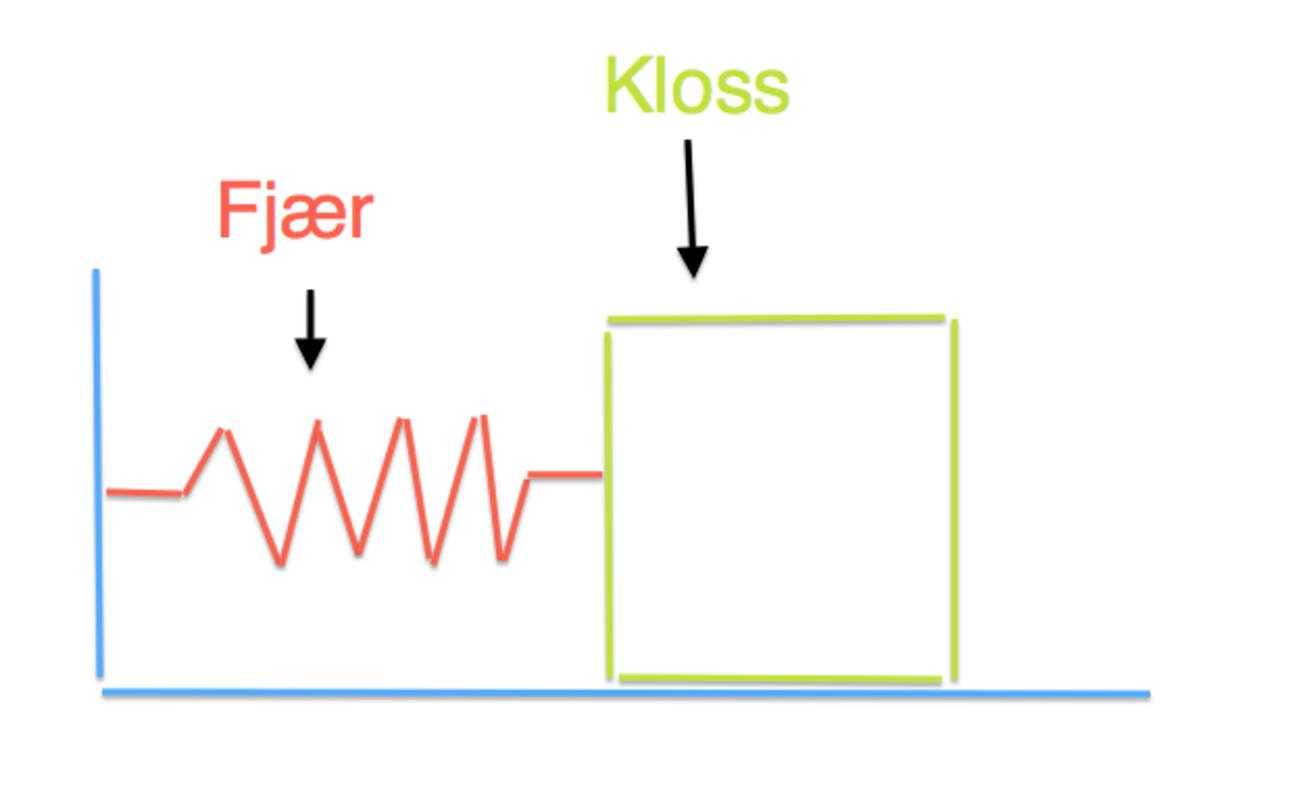
\includegraphics[scale=.35]{Hooke.pdf}
	\label{fig:Num1}
	\end{center}
\end{figure}
\[
F(y)=-ky,
\]
der $y$ er hvor langt fj{\ae}ren er strukket eller komprimert, 
$k$ er en konstant som avhenger av fj{\ae}rens stivhet, 
og $F(y)$ er kraften fra fj{\ae}ren p{\aa} klossen. 
Dersom $y(t)$ er klossens posisjon, er klossens akselerasjon gitt ved $y''(t)$,
og Newtons andre lov blir
\begin{equation*}
-ky=my'',
\end{equation*}
der $m$ er klossens masse. Dette er en differensiallikning. Vi skriver vanligvis
\[
my''+ky=0.
\]

Vi kan komplisere det litt til. La oss innf{\o}re luftmotstand. Luftmotstand avhenger kvadratisk av farten:
\begin{equation*}
F(y')=b(y')^{2};
\end{equation*}
der $b$ er en proporsjonalitetskonstant som sier noe om luftmotstanden. 
Den totale kraften blir
\begin{equation*}
F(y,y')=-ky+b(y')^{2},
\end{equation*}
slik at Newtons andre lov gir
\begin{equation*}
my''-b(y')^{2} +ky=0.
\end{equation*}
Denne likningen har et problematisk ledd, $b(y')^{2}$. Men vi kan gjøre en forenkling. 
Dersom klossen ligger i en tyktflytende væske, blir motstanden proporsjonal med farten istedet for kvadratet av farten, 
og vi får likningen
\begin{equation*}
my''-cy' +ky=0,
\end{equation*}
som er mye enklere å løse.



N{\aa} skal vi komplisere det enda litt. La klossen henge fra taket.
\begin{figure}[htbp]
  \begin{center}
	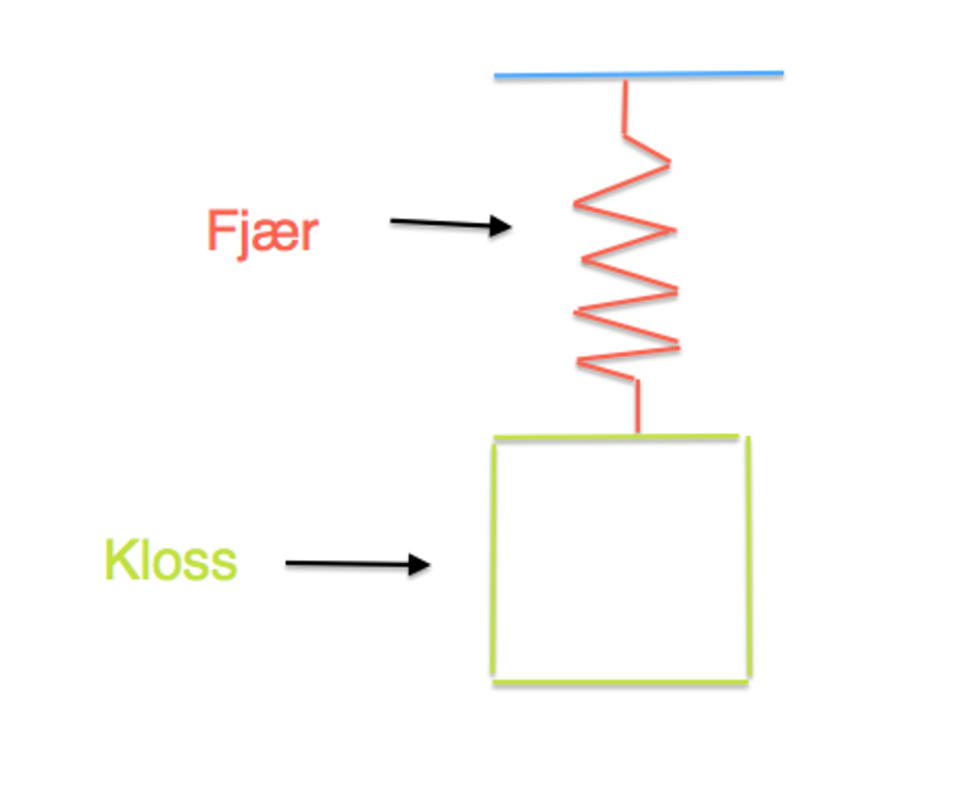
\includegraphics[scale=.4]{Hooke_2.pdf}
	\label{fig:Num1}
	\end{center}
\end{figure}
I tillegg til fj{\ae}rkraften og luftmotstanden, vil n{\aa} ogs{\aa} gravitasjonen p{\aa}virke bevegelsen. Gravitasjonskraften er en konstant kraft $mg$ nedover. Den totale kraften
er
\begin{equation*}
F(y,y')=-ky+by'-mg,
\end{equation*}
og Newtons andre lov gir differensiallikningen
\begin{equation*}
my''-by' +ky=mg.
\end{equation*}



\section*{Noen småting}
Vi skal behandle \defterm{andre ordens differensiallikninger med konstante koeffisienter}:
\[
a_2y''(t)+a_1y'(t)+a_0y(t)=f(t)
\]
Det er vanlig å sette $a_2=1$, for å forenkle analysen. 
Vi slipper å ha med $a_2$ i alle formler og utledninger, og vi slipper å luke ut $a_2=0$ hver gang vi skal sette opp et teorem. 
Dersom $a_2$ skulle slumpe til å være noe annet enn 1, kan du dele den ut av likningen før du setter igang.

Det er tradisjonelt og praktisk å sortere likninger i to kategorier, de homogene:
\[
y''(t)+a_1y'(t)+a_0y(t)=0
\]
og de inhomogene:
\[
y''(t)+a_1y'(t)+a_0y(t)=f(t)
\]




\section*{Løsningsteknikk for homogene likninger}

Vi kaller gjerne løsningen av 
\[
y''(t)+a_1y'(t)+a_0y(t)=0
\]
for $y_h$, der $h$-en står for homogen.
Det første man kan merke seg, er at vi har allerede lært å løse denne typen likning i forrige kapittel. 
Dersom vi innfører de nye variablene $v_1=y$ og $v_2=y'$, kan likningen skrives om til systemet
\[
\begin{bmatrix}
0 & 1 \\ -a_0 & -a_1
\end{bmatrix}
\begin{bmatrix}
v_1 \\ v_2
\end{bmatrix}
=
\begin{bmatrix}
v_1 \\ v_2
\end{bmatrix}'
\]
Vi vet derfor at vi kan forvente to lineært uavhengige løsninger. Det karakteristiske polynomet til matrisen er:
\[
\lambda^2+a_1\lambda + a_0.
\]
Egenvektoren til $\lambda$ er:
\[
\V x=
\begin{bmatrix}
1 \\ \lambda
\end{bmatrix}.
\]

Den karakteristiske likningen kjenner du forhåpentligvis igjen fra gymnaset, der du lærte å løse disse likningene. 
Den gang sa de noe sånt som at alle løsninger var på formen $Ae^{\lambda t}$, og
så satte de dette uttrykket inn i differensiallikningen for å utlede den karakteristiske likningen. 

Vi kan bruke analysen fra forrige oppgave til å liste opp løsningen til den homogene likningen for forskjellige typer egenverdier. 
Merk at vi er i utgangspunktet kun interessert i $v_1$, og derfor ikke har bruk for egenvektorene når vi skal skrive opp løsninger.

Dersom $\lambda_1 \neq \lambda_2$ er reelle, kan vi plukke ut førstekomponenten av den generelle løsningen av systemet, og få
\[
y_h(t)=c_1e^{\lambda_1 t}+c_2e^{\lambda_2 t}.
\]

Dersom $\lambda=\alpha \pm \beta i$, slik at 
\[
\begin{bmatrix}
a_1 \\ a_2
\end{bmatrix}
=
\begin{bmatrix}
1 \\ \alpha
\end{bmatrix}
\]
og
\[
\begin{bmatrix}
b_1 \\ b_2
\end{bmatrix}
=
\begin{bmatrix}
0 \\ \beta
\end{bmatrix},
\]
får vi 
\begin{align*}
y_h(t)=d_1e^{\alpha t}\cos\beta t+d_2e^{\alpha t}\sin\beta t.
\end{align*}

Dersom $\lambda_1=\lambda_2=\lambda$, kan vi stokke litt om på verdiene til $c_1$ og $c_2$, og få
\[
y_h(t)=c_1e^{\lambda t}+c_2te^{\lambda t}.
\]

\begin{ex}
Løsningen til 
\[
y''-y=0
\]
er
\[
y(t)=c_1e^t+c_2e^{-t}. \qedhere
\]
\end{ex}


\begin{ex}
Løsningen til 
\[
y''+y=0
\]
er
\[
y(t)=c_1\cos t+c_2\sin t. \qedhere
\]
\end{ex}

\begin{ex}
Løsningen til 
\[
y''-2y'+y=0
\]
er
\[
y(t)=c_1e^t+c_2te^t. \qedhere
\]
\end{ex}


\section*{Løsningsteknikk for inhomogene likninger}
Tilsvarende kalles vi løsningen til
\[
a_2y''(t)+a_1y'(t)+a_0y(t)=f(t)
\]
for $y_p$, der $p$ står for partikulær. Vi gjør som vi pleier når vi lærer dere å løse likninger, og forteller enkelt og greit hva $y_p$ er. 
La $y_h=y_1+y_2$, der $y_1$ og $y_2$ være to lineært uavhengige homogene løsninger. 
Da er
\begin{align*}
y_p(t)&=y_2\int \frac{y_1(t)f(t)}{y_1(t)y'_2(t)-y_2(t)y'_1(t)}\; dt \\ &-y_1\int \frac{y_2(t)f(t)}{y_1(t)y'_2(t)-y_2(t)y'_1(t)}\; dt.
\end{align*}
Integrasjonskonstanten i de ubestemte integralene skal være 0. 
Denne teknikken kalles \defterm{variasjon av parametre}.

\begin{ex}
Den homogene løsningen til 
\[
y''-y=e^{2t}
\]
er
\[
y_h(t)=c_1e^t+c_2e^{-t}=c_1 y_1(t)+c_1 y_2(t),
\]
slik at 
\begin{align*}
y_p(t)&=y_2\int \frac{y_1(t)f(t)}{y_1(t)y'_2(t)-y_2(t)y'_1(t)}\; dt \\ &-y_1\int \frac{y_2(t)f(t)}{y_1(t)y'_2(t)-y_2(t)y'_1(t)}\; dt\\&=e^{-t}\int \frac{e^te^{2t}}{-e^{t}e^{-t}-e^{-t}e^{t}}\; dt \\ &-e^{t}\int \frac{e^{-t}e^{2t}}{-e^{t}e^{-t}-e^{-t}e^{t}}\; dt= \frac{1}{3}e^{2t},
\end{align*}
og
\[
y=y_h+y_p=c_1e^t+c_2e^{-t}+\frac{1}{3}e^{2t}.  \qedhere
\]
\end{ex}


\begin{ex}
Den homogene løsningen til 
\[
y''-y=e^{t}
\]
er
\[
y_h(t)=c_1e^t+c_2e^{-t},
\]
slik at 
\begin{align*}
y_p(t)&=e^{-t}\int \frac{e^te^{t}}{-e^{t}e^{-t}-e^{-t}e^{t}}\; dt \\ &-e^{t}\int \frac{e^{-t}e^{t}}{-e^{t}e^{-t}-e^{-t}e^{t}}\; dt= \frac{1}{2}(t-1)e^{t},
\end{align*}
og
\[
y=c_1e^t+c_2e^{-t}+\frac{1}{2}(t-1)e^{t}.  \qedhere
\]
\end{ex}

\begin{ex}
Den homogene løsningen til 
\[
y''+y=\sin t
\]
er
\[
y_h(t)=c_1\cos t+c_2\sin t,
\]
slik at 
\begin{align*}
y_p(t)&=\sin t \int \frac{\cos t \sin t}{\cos^2 t+\sin^2 t}\; dt \\ &-\cos t \int \frac{\sin^2 t}{\cos^2 t+\sin^2 t}\; dt\\
&=\sin t \int \cos t \sin t\; dt -\cos t \int \sin^2 t\; dt\\
&=-\frac{1}{4}\sin t \cos 2t  -\cos t \left(\frac{t}{2}-\frac{1}{4}\sin 2t\right)\\ 
&= -\frac{1}{2}t\cos t-\sin t. 
\end{align*}
Merk at den homogene løsningen $y_1=\sin x$ dukket opp i prosessen. 
Dette skjer av og til, men gjør ingenting. Vi har 
\[
y=c_1 \cos t + c_2 \sin t - \frac{1}{2}t\cos t. \qedhere
\]
\end{ex}


%
%Vi skal ikke bevise formelen, men registrere at for noen spesialtilfeller kan vi sette opp en tabell.
%For noen enkle høyresider holder det å vite hva $y_p$ skal være for forskjellige $f$, 
%og så må man sette $y$ inn i likningen for å bestemme noen konstanter. Her er en tabell: \\
%
%\begin{tabular}{l l}
%f & y \\
%\hline
%$t^n$ & $ct^n$ \\
%$\sin t$ & $c_1 \cos t + c_2 \sin t$ \\
%$\cos t$ & $c_1 \cos t + c_2 \sin t$ \\
%$e^{at} \quad (a \neq \lambda)$ & $c e^{at} $ \\
%$e^{\lambda t}\quad \lambda$ er ikke dobbel  & $c te^{\lambda t} $ \\
%$e^{\lambda t}\quad \lambda$ er dobbel  & $c t^2e^{\lambda t} $ \\[10pt]
%\end{tabular}
%
%Det finnes noen typer inhomogene likninger som ikke lar seg løse på dette viset, for eksempel når $f(t)=\tan t$, og da må man inn med variasjon av parametre.


\section*{Apoteose}

Til slutt kan vi registrere at den generelle løsningen til 
\[
a_2y''(t)+a_1y'(t)+a_0y(t)=f(t)
\]
er
\[
y(t)=y_h(t)+y_p(t).
\]
 Merk at det finnes to ubestemte koeffisienter i $y_h$, så et initialverdiproblem trenger to betingelser - den vanligste formen er 
 \[
 y(t_0)=a, \quad  y'(t_0)=b.
\]

\begin{ex}
Løsningen til initialverdiproblemet
\[
y''-y=e^{2t}
\]
med betingelser
 \[
 y(0)=1, \quad  y'(0)=0
\]
er
\[
y=\frac{2}{3}e^{-t}+\frac{1}{3}e^{2t}.  \qedhere
\]
\end{ex}


\kapittelslutt
